\section{Code manual}
In this section the code will be explained into detail, such that an user who is familiar with MATLAB can operate the code. 

\subsection{Data storage}
In the beginning of the main code 2 path's, directing to a file in the results folder, is created to store the results. One file contains the data for the retenate and the other for the permeate. The piece of code that executes this task is shown below:

\begin{lstlisting}[firstnumber={17}]
%% set path to folder where values must be stored, clean the old file
path_Results1 = 'C:\Users\s137280\Documents\Master_tue\Internship\internship_github\ Toos_simplified_species_v02_02_2019\results\retenate.txt';
path_Results2 = 'C:\Users\s137280\Documents\Master_tue\Internship\internship_github\ Toos_simplified_species_v02_02_2019\results\permeate.txt';

% add name taggs to created file and close file again.
test = fopen(path_Results1,'w');
fprintf(test,'%-12s %-12s %-12s %-12s %-12s %-12s %-12s \n', 'Time','Position', 'u_Position', 'X1', 'X2', 'X3','X4');
fclose(test);

% add name taggs to created file and close file again.
test = fopen(path_Results2,'w');
fprintf(test,'%-12s %-12s %-12s %-12s %-12s %-12s %-12s\n', 'X2_1', 'X2_2', 'X2_3', 'X2_4', 'stagecut');
fclose(test);
\end{lstlisting}

At specific times, declared in the array \textit{store\_times}, the data is stored in the files 'retenate.txt' and 'permeate.txt'. In this case the time, position, velocity-position and mole fraction of the retenate are stored in 'retenate.txt'. The stagecut and mole fraction of the permeate are stored in 'permeate.txt'. More variables could be stored as long as they have the same dimensions. Note, the variable must be added in the part above and below. 
   
\begin{lstlisting}[firstnumber={120}]
%     store data at different time steps
if time == store_times(ii)
time_x = time*ones(1,length(u));
file1 = fopen(path_Results1,'a');
fprintf(file1,'%-12.6f %-12.6f %-12.6f %-12.6f %-12.6f %-12.6f %-12.6f \n',[time_x; x; x_u; X_k(1,:); X_k(2,:); X_k(3,:); X_k(4,:)]);    
fprintf(file1,'\n');        
fclose(file1);

file2 = fopen(path_Results2,'a');
fprintf(file2,'%-12.12f %-12.12f %-12.12f %-12.12f %-12.12f %-12.12f %-12.12f\n',[X2_k(1,:); X2_k(2,:); X2_k(3,:); X2_k(4,:); theta]);    
fprintf(file2,'\n');        
fclose(file2);        

ii = ii +1;
end
\end{lstlisting} 
\subsection{Initializing variables}
Part of the variables are initialized in the main code. Other variables, especially variables that can have a different value for every grid cell, are initialized upon use of a function. First, the initialization in the main code will be explained, followed by an explanation of the functions \textit{species\_init()} and \textit{param\_init()}. 
\subsubsection{Variables in main code}
Next step is to initialize a set of variables. The following set of variables are declared in the main code. The meaning of each variable is written behind it as a comment, with it's corresponding unit. 

\begin{lstlisting}[firstnumber={34}]
%% initializing
global Patm Runiv      
Patm        = 101325;       % athmosphesric pressure 				[Pa]
Runiv        = 8.314;		% universal gas constant 				[J/mol.K]

NPI         = 200;          % number of grid cells in x-direction 	[-] 
XMAX        = 1;            % length of the domain 					[m]
u_in        = 1;            % inflow velocity 						[m/s]
T           = 298;          % temperature 							[K]
A           = 1;            % area of one cell 						[m^2]
Total_time  = 200;          % total simulation time 				[s]
Pr          = 400*10^3;     % pressure retenate 					[Pa]
Pp          = 40*10^3;      % pressure permeate 					[Pa]
w           = 1;            % width of cell domain 					[m]
\end{lstlisting}

\newpage
\subsubsection{Species\_init()}
The species parameters are initialized with a separate function called '\textit{species\_init()}'. This function requires the number of grid cells, NPI, as an input and it returns:
\begin{itemize}
	\item \textit{rho\_s}, the density of the individual species 
	\item \textit{rho}, an artificial density required for computation
	\item \textit{Gamma} and \textit{Gamma\_k}, thermal diffusion coefficient of the individual species and thermal diffusion coefficient at the retenate side. 
	\item \textit{MW\_mix} and \textit{MW2\_mix}, the molar weight of the mixture at the retenate and permeate side. 
	\item \textit{Y\_k} and \textit{X\_k}, the mass and mole fraction at the retenate side.
	\item \textit{Y\_in} and \textit{X\_in}, the inlet composition at the retenate side in terms of mass fractions and mole fractions. 
	\item \textit{Y2\_k} and \textit{X2\_k}, the mass and mole fraction at the permeate side.
	\item \textit{Y2\_in} and \textit{X2\_in}, the inlet composition at the permeate side in terms of mass fractions and mole fractions. 
	\item \textit{iAll}, a matrix containing the numbers of species of interest to get data from a MechanismFile, which is included in the same folder as the code.  
	\item \textit{MW}, the molar weight of the individual species. 
	\item \textit{rho\_real} and \textit{rho2\_real}, the real density at the retenate and permeate side. 
	\item \textit{rho\_old} and \textit{rho2\_old}, the old real density at the retenate and permeate side. 	
	\item \textit{D}, \textit{D\_k} and \textit{D2\_k}, the diffusion coefficient of the individual species into another species and the average diffusion coefficient at each cell for the retenate and permeate side.
	\item \textit{P\_k}, the permeability of the individual species.
	\item \textit{f\_old} and \textit{f2\_old}, the old mass fraction at the retenate and permeate side. 	
	\item \textit{sink}, a vector which indicates which species will leak and which not. A zero represent no leakage and a one represents leakage.
	\item \textit{n}, the number of species used in the computation.
\end{itemize}
 
\begin{lstlisting}[firstnumber={49}]
% species properties some values have to be set manually!!
[rho_s, rho,Gamma, Gamma_k, MW1, MW2, Y_k, X_k, Y_in, X_in, Y2_k, X2_k, Y2_in, X2_in, iAll, MW, rho_real, rho2_real, rho_old, rho2_old, D, D_k, D2_k, P_k, f_old, f2_old, sink, n] = species_init(NPI);
\end{lstlisting}

Note that the permeate side has not a real inlet condition, \textit{Y2\_in}, this variable is only used to make sure that this side is initialized with a certain mixture. The composition at the permeate side can only change due to permeation which is modelled as a source term and will be explained later. If no permeation would occur, there is no fluid flow at the permeate side and no change in composition. \\
\\
The next code snippet contains the script of the function \textit{species\_init()}.
\newpage
\begin{lstlisting}
function [rho_s, rho,Gamma, Gamma_k, MW_mix, MW2_mix, Y_k, X_k, Y_in, X_in, Y2_k, X2_k, Y_in2, X_in2, iAll, MW, rho_real, rho2_real, rho_old, rho2_old, D, D_k, D2_k, P_k, f_old, f2_old, sink, n] = species_init(NPI)

	%% Read species data
	% Make these variable global
	global El Sp Patm Runiv

	MechanismFile = 'fuels.trot';

	% Read the reaction mechanism
	[El, Sp] = ReadTrotDat(MechanismFile);

	%% Define some species
	iO2   = find(strcmp({Sp.Name},'O2'));
	iCO2  = find(strcmp({Sp.Name},'CO2'));
	iH2O  = find(strcmp({Sp.Name},'H2O'));
	iAr   = find(strcmp({Sp.Name},'AR'));

	iAll  = [iO2 iCO2 iH2O iAr];

	MW   = [Sp(iAll).Mass];                  % Molar weight of species [gr/mol]
	n = length(iAll);

	%% mole flow rate in system and sink term
	moles = [1.541694; 10.329175; 0.973272;  87.155861];
	moles2 =[0  ;  0 ; 0 ; 1];    % code will crash if everything is set to 0

	X_in  = moles/sum(moles);
	X_in2 = moles2/sum(moles); 

	sink  = [1  1  1  1];         % this array can prevent species from leakage
	P_n   = [28; 350; 1750; 21]*10^(-9);  % Permeability of species

	Gamma = [ThermProp(300,Sp(iO2),'Gamma','Mass') ThermProp(300,Sp(iCO2),'Gamma','Mass') ThermProp(350,Sp(iH2O),'Gamma','Mass') ThermProp(350,Sp(iAr),'Gamma','Mass')];
	rho_s = [1.429 1.98 1.2504 1.784];    % 'Real' density of species [kg/m^3]

	for i = 1:n
		Y(i,:) = X_in(i)*MW(i)/(MW*X_in);                
		Y2(i,:) = X_in2(i)*MW(i)/(MW*X_in2);

	end

	Y_in  = Y(:,1);
	Y_in2 = [0;0;0;0];

	MW1 = MW*X_in;                          % molar weight of mixture    
	MW2 = MW*X_in2;                         % molar weight of mixture    

	D       = species_diff(NPI, 300, iAll, iAll, 'Diffusivity', n); % Diffusivity of species [m^2/s]

	for j = 1:n

		for I = 1:NPI+2
			p_k (j,I)   = Patm;             % pressure of species k
			Y_k(j,I)    = Y(j);             % mass of species k
			Y2_k(j,I)   = Y2(j);            % mass of species k
			MW_k(j,I)   = MW(j);            % molar weight of species k
			P_k(j,I)    = P_n(j);           % Permeability
			X_k(j,I)    = X_in(j);
			X2_k(j,I)   = X_in2(j);
			MW_mix(1,I) = MW1;
			MW2_mix(1,I)= MW2;
		end

	end

	for j = 1:n
		for i = 1:NPI+2
			D_k(j,i) = D(j,:)*Y_k(:,i);    % Diffusion is in terms of mass 
										   % so use massfraction!!
			D2_k(j,i) = D(j,:)*Y2_k(:,i);  % Diffusion is in terms of mass
										   % so use massfraction!! 
			Gamma_k(1,i) = Gamma*Y_k(:,i);
			rho(1,i)    = 1;
			rho_real(1,i) = rho_s*Y_k(:,i);
			rho2_real(1,i) = rho_s*Y2_k(:,i);
		end                                
	end

	f_old = Y_k;
	f2_old = Y2_k;
	rho_old = rho_real;
	rho2_old = rho2_real;

end
\end{lstlisting}
\newpage
\subsubsection{Param\_init()}
With the function \textit{param\_init()} another set of parameters is initialized. This function requires the number of grid cells and inlet velocity, \textit{u\_in}, as input and returns:

\begin{itemize}
	\item \textit{u}, the initial velocity at the retenate side.
	\item \textit{u2}, the initial velocity at the permeate side.
	\item \textit{relax\_f}, relaxation factor for the computation of the new mass fraction of the species.
	\item \textit{Dt}, time step size 
\end{itemize}

\begin{lstlisting}[firstnumber={52}]
% make a vector with initial values for all non-specie dependent parameters 
[u, u2, relax_f, Dt] = param_init(NPI, u_in);
\end{lstlisting}
Below the script is given of the function \textit{param\_init}. 
\begin{lstlisting}
function [u, u2, relax_f, Dt] = param_init(NPI, u_in);
	Dt = 0.5;
	for I=1:NPI+2
		i = I;
		u(i)    = u_in;         % Velocity in x-direction
		u2(i)   = 0;
	end

	relax_f = 1;              % relaxation for temperature
end
\end{lstlisting}

\section{Grid generation}
A 1D staggered grid is created with the function \textit{grid\_gen()}. A staggered grid is a setting in which the discretised variables are not defined at the same position. Typically, the velocity is defined at cell faces and all other variables are defined at cell centres. The main benefit of the staggered grid is that it does not result in the decoupling of pressure and velocity, leading to the checkerboard problem. In Figure \ref{fig:fig9} a picture of a staggered grid is shown. Note, two different notations are used in this figure to describe the cell faces and centres. The variables I, referring to cell centres, and i, referring to cell faces, with i = 0,1,2,...,N+2 and I = 0,1,2,...,N+2 is more generic. The use of W, P, E and w, e, p, is more convenient to describe the discretised equations.  

\begin{figure}[H]
	\centering
	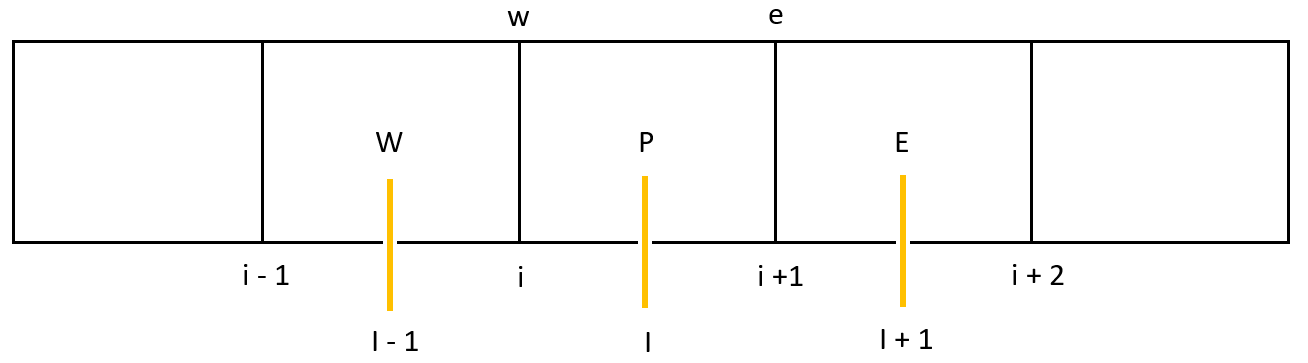
\includegraphics[width= 1\textwidth]{Images/fig1.png}
	\captionof{figure}{Discretised staggered grid.}
	\label{fig:fig9}
\end{figure}
The use of a staggered grid is not necessary for this particular case since pressure and velocity don't change. However, the staggered grid was implemented at an early stage of the project and for future improvements it is more convenient to use the staggered grid. At this stage the use of a staggered grid has no influence on the results.  \\

The function \textit{grid\_gen()} requires the number of grid cells and the length of the domain, \textit{XMAX}, as input. It returns:
\begin{itemize}
	\item \textit{Dx}, the distance between two grid cells/ faces.
	\item \textit{x} the positions where all variables except velocity are defined.  
	\item \textit{x\_u}, the positions where velocity is defined. 
\end{itemize}

\begin{lstlisting}[firstnumber={55}]
	%% grid generation
	[Dx, x, x_u] = grid_gen(NPI,XMAX);      % create staggered grid
\end{lstlisting} 

The script of the function \textit{grid\_gen()} is shown below. If the user would like to decrease the grid spacing, \textit{Dx}, this should be done by increasing the parameter \textit{NPI}, which is declared at the beginning of the main code. Also, if the grid should be longer, this should be modified by increasing the value for \textit{XMAX} which is also declared at the beginning of the main code.
\begin{lstlisting}
function [Dx, x, x_u] = grid_gen(NPI, XMAX)
	% Length of the element
	Dx = XMAX/NPI;
	x(1) = 0;
	x(2) = 0.5*Dx;
	
	% Length variable for the scalar points in the x direction
	for I=3:NPI+1
		x(I) = x(I-1)+Dx;
	end
	x(NPI+2) = x(NPI+1) + 0.5*Dx;

	% Length variable for the velocity components u[i] in the x direction
	% Used to make staggered grid
	x_u(1) = 0;
	x_u(2) = 0;
	for i=3:NPI+2
		x_u(i) = x_u(i-1)+Dx;
	end   
end
\end{lstlisting}

